\section{Orientaci\'on al arco}

Al finalizar la búsqueda de la pelota, se desea poder patearla con dirección al arco. El procedimiento para la búsqueda del arco es an\'alogo al procedimiento de la b\'usqueda de la pelota explicado en la sección \ref{sec:busqueda}.
Se tiene la representación del mundo dividida en regiones como se muestra en la figura ~\ref{divisionCamArco}. Los recuadros negros representan la imagen captada por las posiciones de la cámara (a) (c) y (e) que se muestran en la imagen de la figura ~\ref{posicionesCam}. En esta ocasi\'on se cuenta con 8 estados. Siete de ellos cuando el arco se detecta en alguna de las regiones y el último estado representa la ocasión en la que no se encuentra el arco. 
A diferencia de la representaci\'on cuando se busca la pelota en esta se reducen los tres movimientos de la c\'amara por dos razones principales. En primera instancia las acciones eliminadas apuntan al suelo y el arco no puede encontrarse en el suele, la segunda raz\'on es que el arco es en proporci\'on mucho mas grande que la pelota por eso la divisiones de las regiones tan presisas como en el caso de la pelota son innecesarias.
\begin{figure}[hbtp]
\centering
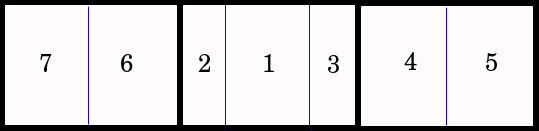
\includegraphics[scale=0.5]{imagenes/RegionesArco.jpg}
\caption{Campo de visión del robot con el número de cada región para buscar el arco. }
\label{divisionCamArco}
\end{figure}

Primero se busca detectar el arco y posicionarse frente a él intentando rodear la pelota, luego se verifica que a\'un la pelota se encuentre en la zona de pateo y se procede a patear hacia el arco.

Las acciones que se toman en cada regi\'on se especifican a continuación: 
 \begin{itemize}

\item Cuando el arco esta a la izquierda de Junny este debe girar a la izquierda esto sucede en las regiones 2, 6, 7, con esto se centra con respecto al arco logra tener un mayor angulo de patada al arco.

\item Cuando el arco esta a la derecha de Junny este debe girar a la derecha esto sucede en las regiones 3, 4 y 5, con esto se centra con respecto al arco y tener mayor angulo de patada al arco.


\end{itemize}

Cuando el arco se encuentra en la regi\'on 1. Se da por finalizada la búsqueda y posicionamiento frente al arco.  

Para lograr el ajuste adecuado cuando Junny encuentra el arco y debe colocarse en posici\'on de pateo los movimientos que debe realizar su cadera no lo permite pues necesita un grado de libertad m\'as para lograrlo, este grado de libertad fue eliminado al principio del proyecto debido a ciertos problemas con los motores Dynamixel los cuales debido al uso constante y exigente suelen fallar y quemarse, la mayor\'ia de estos motores se quemaron justamente en la zona de la cadera. De igual manera los experimentos de desempe\'~no que incluyen patear al arco se realizaron y se presentan en el cap\'itulo ~\ref{chapter:resultados}.






